\documentclass[graphics]{beamer}

\usepackage{graphicx}
\usepackage{verbatim}
\usepackage{wrapfig}
\useoutertheme{shadow}
%\usecolortheme{orchid}
\usecolortheme{seahorse}


% math commands
\newcommand{\be}{\begin{eqnarray}}
\newcommand{\ee}{\end{eqnarray}}
\newcommand{\beq}{\begin{equation}}
\newcommand{\eeq}{\end{equation}}
\def\simless{\mathbin{\lower 3pt\hbox
      {$\rlap{\raise 5pt\hbox{$\char'074$}}\mathchar"7218$}}}
\def\simgreat{\mathbin{\lower 3pt\hbox
      {$\rlap{\raise 5pt\hbox{$\char'076$}}\mathchar"7218$}}} %> or of order

% variables

\def\toonscale{0.45}
\def\mboxy#1{\mbox{\small #1}}


\begin{comment}
\AtBeginSection[]{
  \frame{
    \frametitle{Outline}
    \tableofcontents[currentsection]
  }
}
\end{comment}

\title{FRB as coherent probes
}
%\subtitle{interim update}
\author[U. Pen]{Ue-Li Pen
}
\date{August 4, 2021}


\begin{document}

%\section*{Introduction}
\section{Lenses}

\begin{comment}
  \subsection{Outline}

  \frame{
    \frametitle{Outline}
    \tableofcontents
  }
\end{comment}

\frame{\maketitle}



  \frame{
    \frametitle{Lenses}
    \begin{itemize}
        \item FRB: known to be coherent sources (Masui et al 2015,
          FRB110523)
        \item form interference pattern (e.g. Main+ 2108.00052)
        \item Gravitational Lensing: micro, macro
        \item Plasma lensing
        \item use FRB's to probe universe
        \item use lenses to probe FRBs
    \end{itemize}
  }


  \frame{
\vspace{-0.5in}
    \frametitle{Coherence}
    \begin{itemize}
    \item almost all astronomical objects are {\it resolved} under
      multipath propagation
    \item  unresolved {\it coherent} sources exhibit interference
      pattern through multipath propagation
    \item only pulsars and FRBs are known to fully modulate on
      diffractive time scales
    \item observed FRB plasma lensing implies gravitational (micro-)lensing
      (c.f. last week discussion)
    \end{itemize}
  }

\frame{
    \frametitle{Crab}
     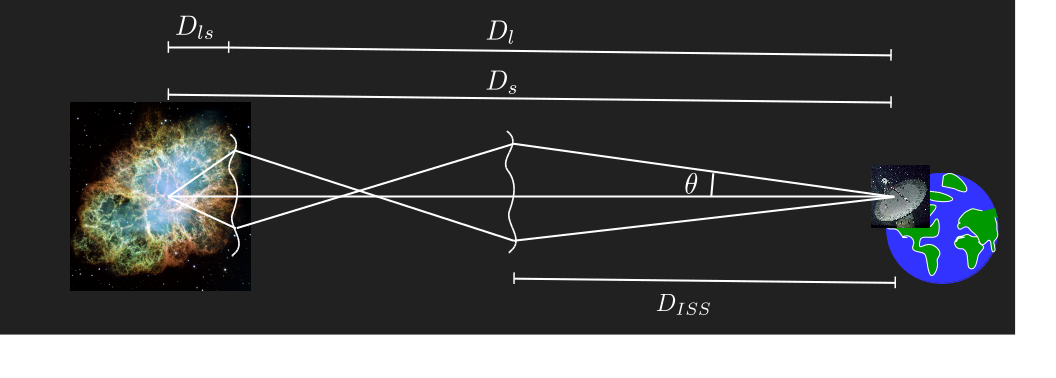
\includegraphics[width=1.1\textwidth]{Figures/TwoScreenGeometry.png}

(figure credit: R. Main)

$\tau_{\rm nebula}\gg \tau_{\rm ISM}$
}


  \frame{
\vspace{-0.25in}
    \frametitle{Initial results}
    \begin{itemize}
        \item FRB110523: use galactic scintillation of scattering tail
          to show that scattering occuring in host, not along the path
        \item FRB201124A: measurement of scintillation time scale/frequency
        \item black widow PSR: direct resolution of emission region
          (Main+2018, Nature, 557, 522)
        \item crab resolving of GP: Main+2021, ApJ 915, 65
        \item crab: evidence for high Lorentz factor $\gamma \sim
          10^4$ with small $\Delta \gamma/\gamma < 0.01$  (2105.08851)
        \item empirical support for $\gamma^2$ free electron laser
          (Lyutikov+ 2021), moving mirror (Colgate+1971)
    \end{itemize}

  }


  \frame{
\vspace{-0.5in}
    \frametitle{New Observables}
    \begin{itemize}
    \item microlensing: instant time delay, planets (Jow+20)
    \item weak lensing: imaginary image allows time delay measurement (Jow+21)
    \item macrolensing: potentially nano-second delay -- universe
      expands! (Wucknitz+21)
    \item dimensionless strain picoseconds/Giga years $h\sim \Delta t/t \sim 10^{-26}$:
      competitive with LIGO, LISA, etc (Yang+2017)
    \item strong lensing: delay measurements enable measurement of
      co-linearity (Jow++21)
    \end{itemize}
\vspace{-0.4in}
\begin{center}
\includegraphics[width=4.1in]{Figures/lensing-VLBI.png}
\end{center}
\vspace{-0.6in}
  }

  \frame{
\vspace{-0.5in}
    \frametitle{Macrolensing}
    \begin{itemize}
    \item Wucknitz+ 2021
    \item alternate approach to cosmography
    \item triangulation: lens model+time delay measurement = $H_0$
    \item weak link has been lens model
    \item Wave optics: time delay observable to nanoseconds
    \item For repeating FRB, dominated by galaxy transverse
      motion. then cosmic expansion
    \item individual macrolens images split into microlens images by stars
    \end{itemize}
  }



  \frame{
\vspace{-0.5in}
    \frametitle{Discussion}
    \begin{itemize}
    \item Eikonal effects applicable to compact radio sources,
      e.g. FRBs, pulsars
    \item full wave
effect dominates for long wavelengths as Fresnel scale is bigger then Einstein radius
    \item down to planet size
    \item gravitational waves:  LIGO, LISA, PTA
    \end{itemize}
  }



  \frame{
\vspace{-0.5in}
    \frametitle{Current status}
    \begin{itemize}
    \item Eikonal: pulsar scintillation, wind magnification (Main+ 2018)
    \item full wave optics: pulsar wind lensing, solar wind (IPS)
    \end{itemize}
  }

\frame{
    \frametitle{Microscope}
     \vspace{-0.65in}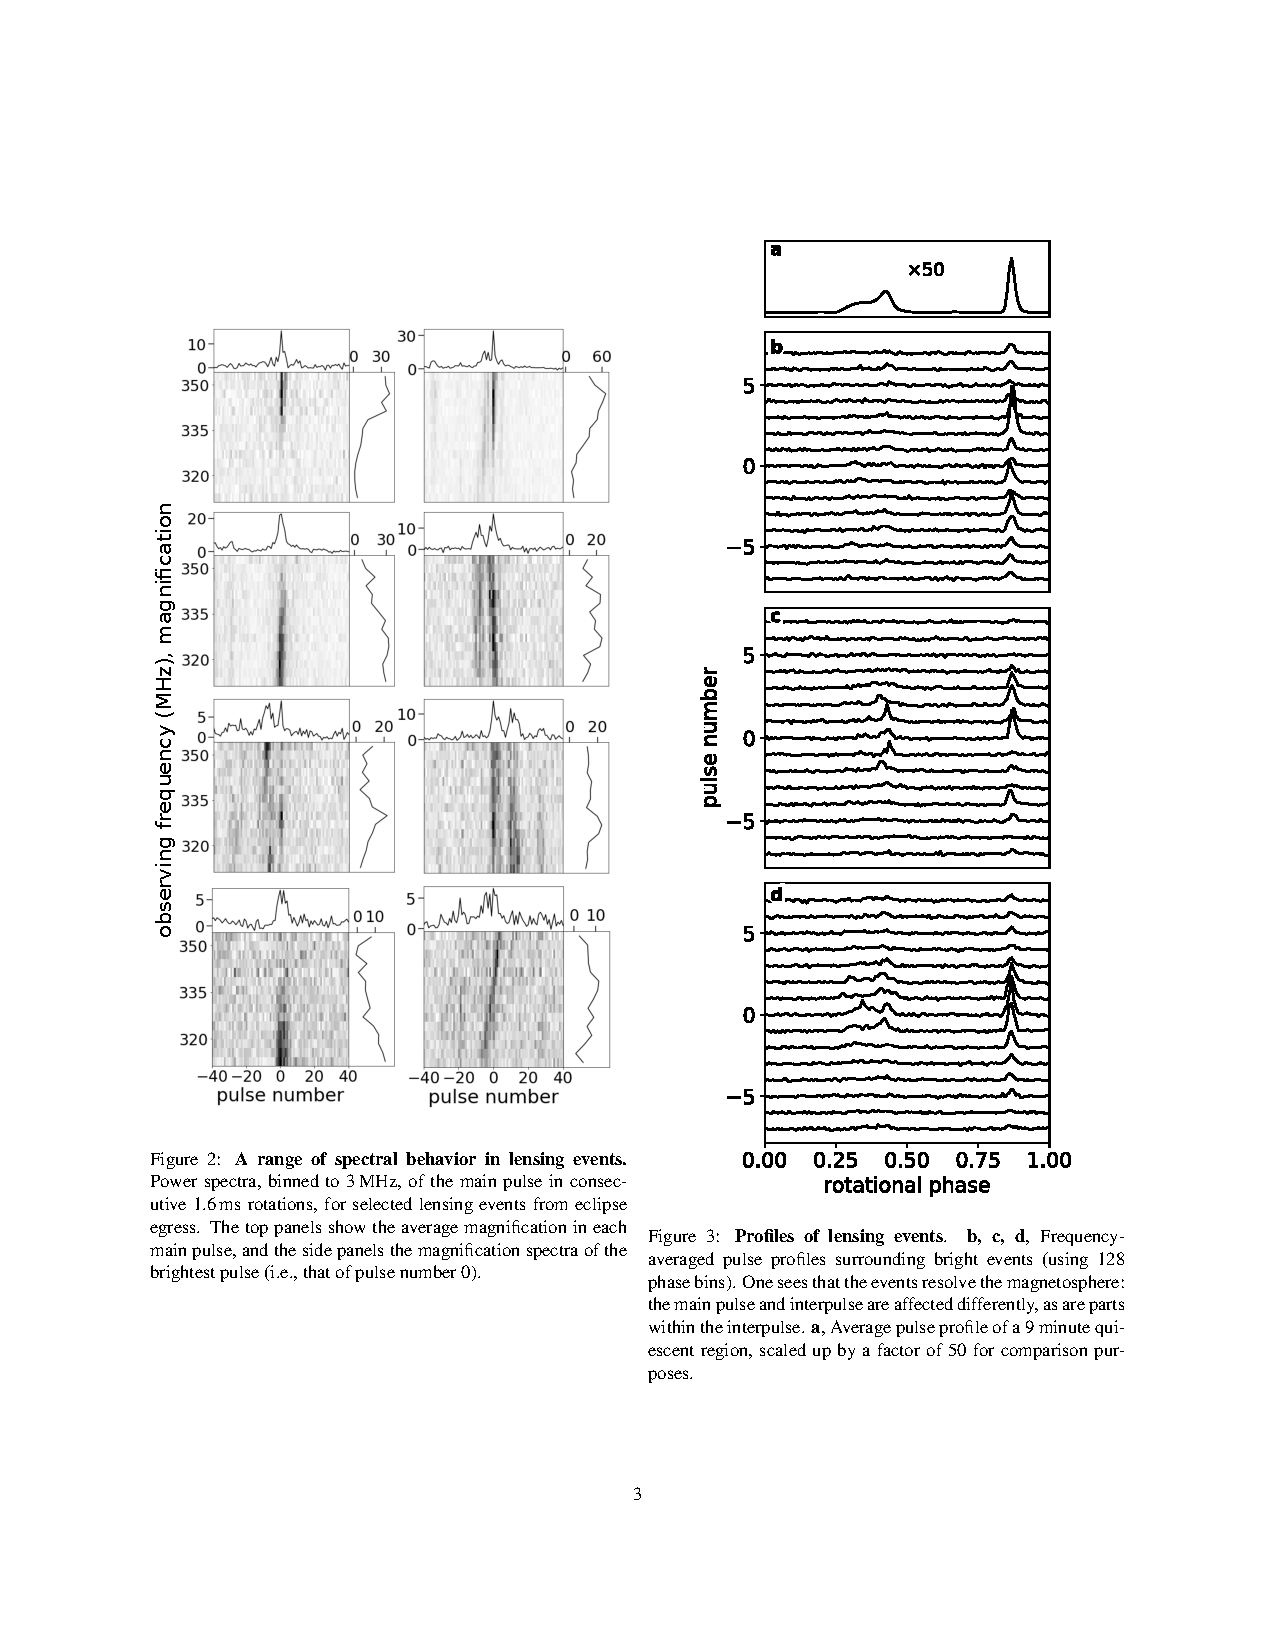
\includegraphics[width=0.75\textwidth]{Figures/bwlens.pdf}
}



  \frame{
\vspace{-0.5in}
    \frametitle{Conclusions}
    \begin{itemize}
    \item wave optics changes nature of observables: one of the potentially most
      precise measurements in physics
    \item coherent radio waves (FRBs, pulsars): described by Eikonal
      away from caustics/catastrophies
    \item crab lensing probe: search for scattered, narrow band,
      drifting FRBs
    \item published studies demonstrate FRB coherence under plasma
      lensing, also for scattered FRB.  More work needed to quantify
      broad samples.
    \item VLBI scintillometry of FRBs and pulsars (e.g. CHIME-outrigger, CHORD)
    \end{itemize}
  }

\end{document}
